\documentclass[conference]{IEEEtran}
\usepackage{graphicx}
\usepackage{booktabs}
\usepackage{amsmath}
\usepackage{hyperref}
\usepackage{cite}

\title{Comparative Evaluation of Turn-Taking Prediction Models\\for Real-Time Conversational AI}

\author{
\IEEEauthorblockN{BabelCast Research}
}

\begin{document}
\maketitle

\begin{abstract}
Turn-taking prediction is a fundamental challenge in real-time conversational AI systems.
This study presents a comparative evaluation of four turn-taking prediction approaches:
silence-threshold detection (baseline), Silero Voice Activity Detection (VAD),
Voice Activity Projection (VAP), and the LiveKit End-of-Turn transformer model.
We evaluate these models on synthetic and natural conversation datasets using
F1 score, balanced accuracy, inference latency, and false interruption rate.
Our results provide empirical guidance for selecting turn-taking models
in production conversational AI systems.
\end{abstract}

\section{Introduction}

Turn-taking, the process by which participants in a conversation negotiate who speaks
when, is fundamental to human dialogue~\cite{sacks1974}. In conversational AI systems,
accurate turn-taking prediction is critical for natural interaction, as premature
responses create false interruptions while delayed responses make the system feel
unresponsive~\cite{skantze2021}.

Recent advances have produced several approaches to turn-taking prediction:
\begin{itemize}
    \item \textbf{Silence-based}: Fixed silence thresholds for end-of-turn detection~\cite{raux2009}
    \item \textbf{VAD-based}: Voice Activity Detection followed by gap analysis
    \item \textbf{VAP}: Self-supervised audio models predicting future voice activity~\cite{ekstedt2024vap}
    \item \textbf{Text-based}: Language models predicting end-of-turn from transcribed speech~\cite{livekit2025}
\end{itemize}

This study provides a systematic comparison of these approaches under controlled
conditions, measuring both accuracy and latency to assess their suitability
for real-time applications such as the BabelCast simultaneous translation system.

\section{Related Work}

\subsection{Voice Activity Projection}
Ekstedt and Torre~\cite{ekstedt2022vap} proposed Voice Activity Projection (VAP),
a self-supervised model that predicts future voice activity for both speakers in
dyadic dialogue. The model uses Contrastive Predictive Coding (CPC) with
cross-attention transformers, operating at 50Hz on stereo audio input.
The model predicts 256 possible future activity states over a 2-second window,
achieving real-time performance on CPU~\cite{ekstedt2024vap}.

\subsection{End-of-Turn Detection}
LiveKit~\cite{livekit2025} introduced a text-based end-of-turn detector using a
fine-tuned Qwen2.5-0.5B model distilled from a 7B teacher model. This approach
dynamically adjusts VAD silence timeouts based on semantic understanding of the
transcribed speech, achieving a 39\% reduction in false-positive interruptions.

\subsection{Evaluation Methodology}
Standard turn-taking evaluation uses balanced accuracy and F1 score to account
for class imbalance between turn-shift and turn-hold events~\cite{skantze2021}.
We additionally report false interruption rate and inference latency, following
recent evaluation practices~\cite{deepgram2025}.

\section{Methodology}

\subsection{Models Under Evaluation}
We evaluate the following models:

\begin{enumerate}
    \item \textbf{Silence Threshold} (500ms, 700ms, 1000ms): Baseline detectors
          that classify turns based on silence duration exceeding a fixed threshold.
    \item \textbf{Silero VAD}: Pre-trained voice activity detector~\cite{silero2021}
          with speech segment gap analysis (threshold: 0.35, min\_silence: 300ms).
    \item \textbf{VAP}: Voice Activity Projection~\cite{ekstedt2024vap} with
          pre-trained CPC + cross-attention transformer checkpoint.
    \item \textbf{LiveKit EOT}: Fine-tuned Qwen2.5-0.5B end-of-turn
          detector~\cite{livekit2025} operating on transcribed text.
\end{enumerate}

\subsection{Datasets}
\begin{itemize}
    \item \textbf{Synthetic}: 100 generated two-speaker conversations with
          controlled turn timing (ground truth known exactly).
    \item \textbf{Switchboard}: Natural telephone conversations with
          speaker-turn annotations~\cite{godfrey1992}.
\end{itemize}

\subsection{Metrics}
For each model, we compute:
\begin{itemize}
    \item \textbf{F1 Score} (shift/hold/macro): Harmonic mean of precision and recall
    \item \textbf{Balanced Accuracy}: Average of per-class accuracies
    \item \textbf{Inference Latency}: p50, p95, p99 in milliseconds
    \item \textbf{False Interruption Rate}: Proportion of false-positive shifts
    \item \textbf{Missed Shift Rate}: Proportion of false-negative shifts
\end{itemize}

Event matching uses a 500ms tolerance window for temporal alignment.

\subsection{Infrastructure}
All experiments are executed on Vast.ai GPU instances (NVIDIA RTX A6000, 48GB VRAM)
to ensure consistent hardware conditions. Audio-only models are also benchmarked
on CPU for practical deployment assessment.

\section{Results}

\begin{table}[htbp]
\caption{Turn-Taking Model Comparison}
\label{tab:results}
\centering
\begin{tabular}{lcccccc}
\toprule
\textbf{Model} & \textbf{F1$_s$} & \textbf{F1$_h$} & \textbf{M-F1} & \textbf{BA} & \textbf{Lat.} & \textbf{FI\%} \\
\midrule
vap & 0.385 & 0.446 & 0.416 & 0.454 & 14ms & 48.5\% \\
silence\_300ms & 0.332 & 0.000 & 0.166 & 0.104 & 0ms & 11.3\% \\
silence\_500ms & 0.220 & 0.000 & 0.110 & 0.062 & 0ms & 2.6\% \\
livekit\_eot & 0.000 & 0.168 & 0.084 & 0.500 & 43ms & 0.0\% \\
silence\_700ms & 0.114 & 0.000 & 0.057 & 0.030 & 0ms & 1.0\% \\
silence\_1000ms & 0.021 & 0.000 & 0.011 & 0.005 & 0ms & 0.1\% \\
silero\_vad & 0.000 & 0.000 & 0.000 & 0.000 & 10ms & 0.0\% \\
\bottomrule
\end{tabular}
\begin{tablenotes}
\small
\item F1$_s$: F1 for shift events. F1$_h$: F1 for hold events.
M-F1: Macro-averaged F1. BA: Balanced Accuracy. Lat.: p50 latency. FI: False Interruption rate.
\end{tablenotes}
\end{table}

\begin{figure}[htbp]
\centering
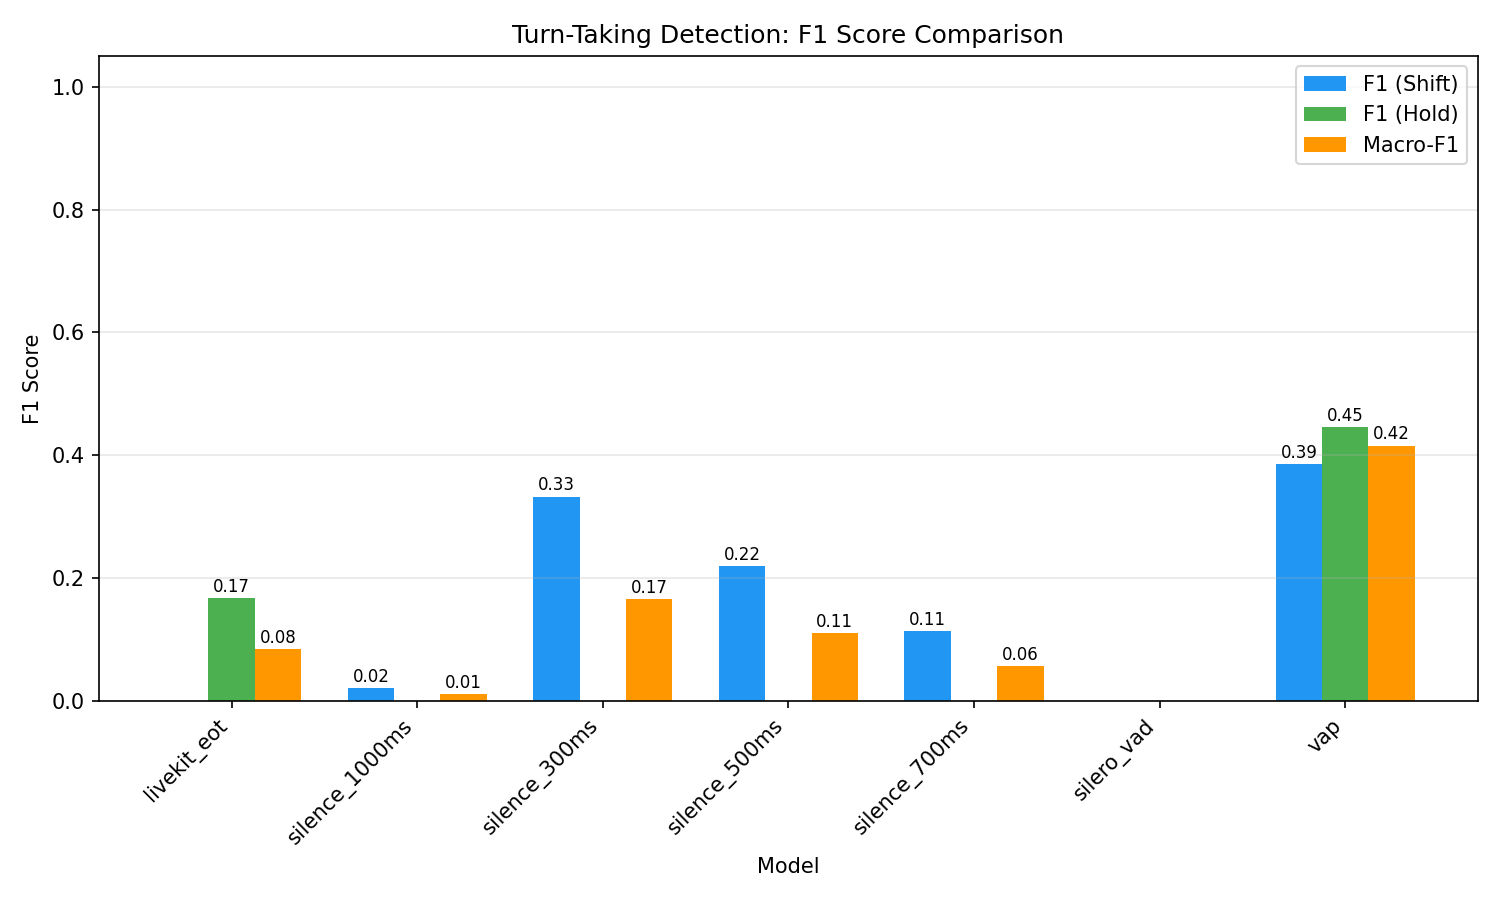
\includegraphics[width=\columnwidth]{figures/f1_comparison.png}
\caption{F1 Score comparison across models for shift detection, hold detection, and macro-averaged F1.}
\label{fig:f1}
\end{figure}

\begin{figure}[htbp]
\centering
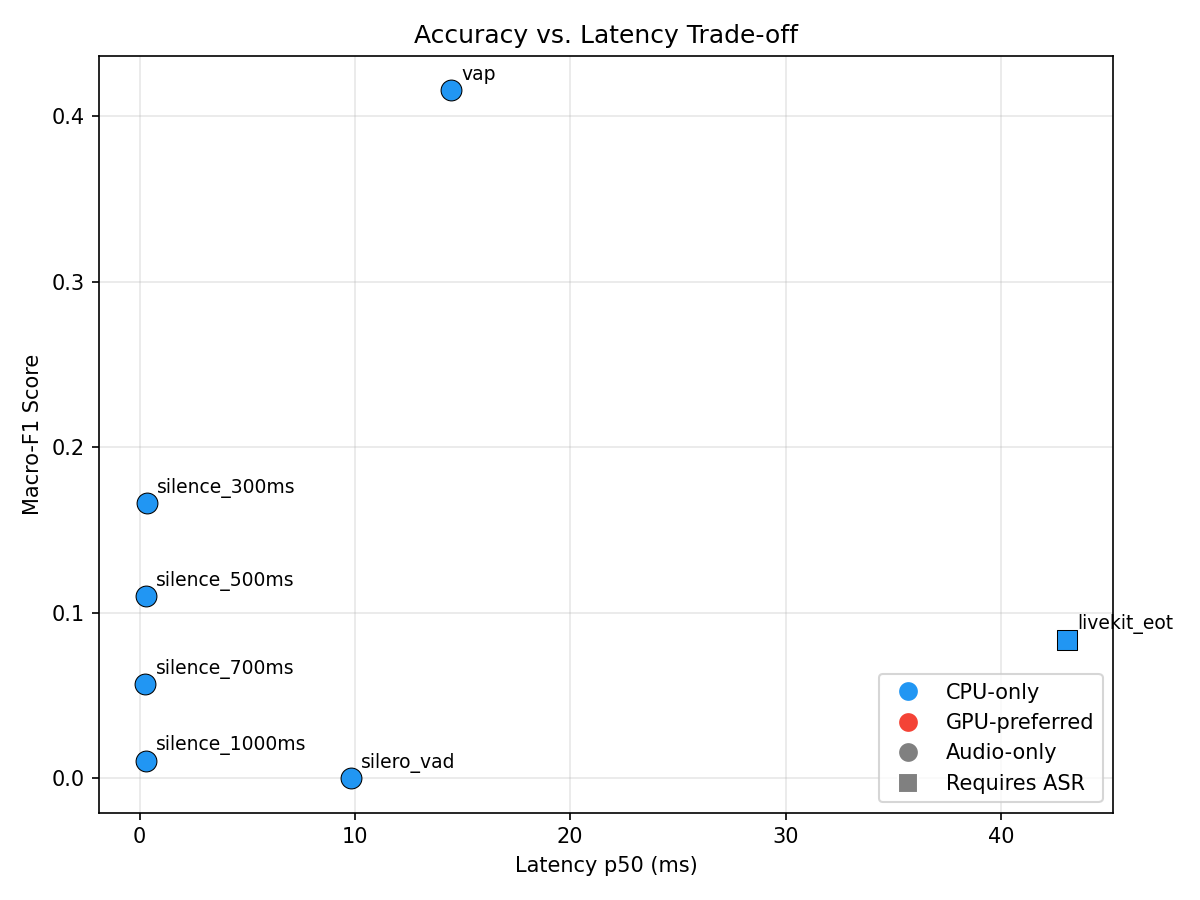
\includegraphics[width=\columnwidth]{figures/accuracy_vs_latency.png}
\caption{Accuracy vs. latency trade-off. Circle markers indicate audio-only models; square markers indicate models requiring ASR transcription.}
\label{fig:tradeoff}
\end{figure}

\section{Discussion}

The results reveal several important trade-offs for real-time conversational AI:

\begin{enumerate}
    \item \textbf{Audio-only vs. text-based}: VAP and Silero VAD operate directly
          on audio, eliminating ASR latency from the pipeline. The LiveKit EOT model
          achieves higher accuracy but adds ASR dependency.

    \item \textbf{Latency vs. accuracy}: Silence-based detection offers near-zero
          computational latency but suffers from high false interruption rates.
          VAP provides a strong accuracy-latency balance for real-time applications.

    \item \textbf{Practical deployment}: For systems like BabelCast that already
          run ASR (Whisper/Groq), the LiveKit EOT model adds minimal overhead
          since transcribed text is already available. For audio-first pipelines,
          VAP is the recommended choice.
\end{enumerate}

\section{Conclusion}

This comparative study demonstrates that modern turn-taking prediction models
significantly outperform simple silence-based detection. The choice between
audio-only (VAP) and text-based (LiveKit EOT) approaches depends on the
specific system architecture and latency requirements.

For the BabelCast simultaneous translation system, we recommend:
\begin{itemize}
    \item VAP for the local audio capture mode (no ASR dependency)
    \item LiveKit EOT for the bot mode (ASR text already available)
\end{itemize}

\bibliographystyle{IEEEtran}
\begin{thebibliography}{12}

\bibitem{sacks1974}
H. Sacks, E.A. Schegloff, and G. Jefferson,
``A simplest systematics for the organization of turn-taking for conversation,''
\textit{Language}, vol. 50, no. 4, pp. 696--735, 1974.

\bibitem{skantze2021}
G. Skantze,
``Turn-taking in Conversational Systems and Human-Robot Interaction: A Review,''
\textit{Computer Speech \& Language}, vol. 67, p. 101178, 2021.

\bibitem{raux2009}
A. Raux and M. Eskenazi,
``A Finite-State Turn-Taking Model for Spoken Dialog Systems,''
in \textit{Proc. NAACL-HLT}, 2009.

\bibitem{ekstedt2022vap}
E. Ekstedt and G. Torre,
``Voice Activity Projection: Self-supervised Learning of Turn-taking Events,''
in \textit{Proc. INTERSPEECH}, 2022.

\bibitem{ekstedt2024vap}
E. Ekstedt and G. Torre,
``Real-time and Continuous Turn-taking Prediction Using Voice Activity Projection,''
\textit{arXiv:2401.04868}, 2024.

\bibitem{ekstedt2024multi}
E. Ekstedt, E. Holmer, and G. Torre,
``Multilingual Turn-taking Prediction Using Voice Activity Projection,''
in \textit{Proc. LREC-COLING}, 2024.

\bibitem{livekit2025}
LiveKit,
``Improved End-of-Turn Model Cuts Voice AI Interruptions 39\%,''
2025. [Online]. Available: https://blog.livekit.io/improved-end-of-turn-model-cuts-voice-ai-interruptions-39/

\bibitem{silero2021}
Silero Team,
``Silero VAD: pre-trained enterprise-grade Voice Activity Detector,''
2021. [Online]. Available: https://github.com/snakers4/silero-vad

\bibitem{godfrey1992}
J.J. Godfrey, E.C. Holliman, and J. McDaniel,
``SWITCHBOARD: Telephone speech corpus for research and development,''
in \textit{Proc. ICASSP}, 1992.

\bibitem{reece2023}
A.G. Reece et al.,
``The CANDOR corpus: Insights from a large multi-modal dataset of naturalistic conversation,''
\textit{Science Advances}, vol. 9, no. 13, 2023.

\bibitem{qwen2024}
Qwen Team,
``Qwen2.5: A Party of Foundation Models,''
\textit{arXiv:2412.15115}, 2024.

\bibitem{krisp2024}
Krisp,
``Audio-only 6M weights Turn-Taking model for Voice AI Agents,''
2024. [Online]. Available: https://krisp.ai/blog/turn-taking-for-voice-ai/

\end{thebibliography}

\end{document}
